\section{Arquitectura y Diseño}

La arquitectura de la aplicación web va a ser de tres capas Modelo-Vista-Controlador, basado en la reutilización de código y separación de componentes, facilitando el desarrollo y mantenimiento de la aplicación.

\begin{figure}[H]
    \centering
    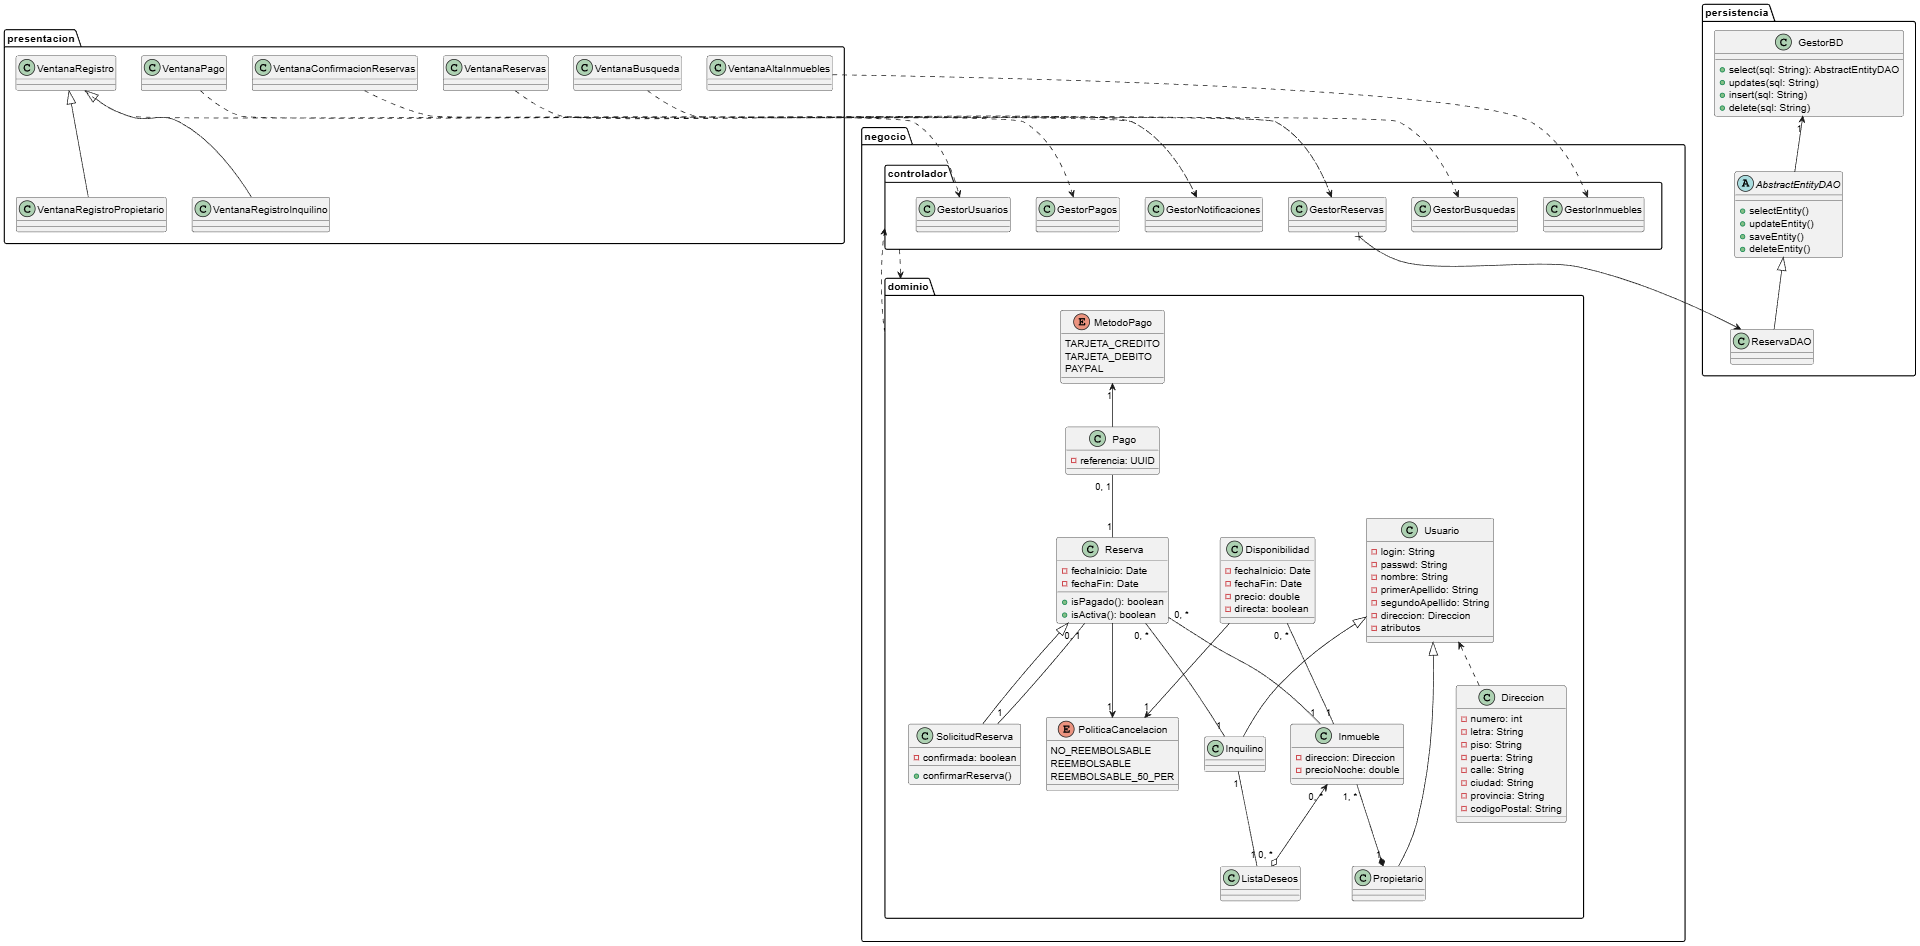
\includegraphics[width=1\linewidth]{img/image.png}
    \caption{Diseño de clases de la aplicación web Bckroom.}
    \label{fig:placeholder}
\end{figure}

Para la persistencia del sistema se utilizará un modelo relacional de base de datos.

\begin{figure}[H]
    \centering
    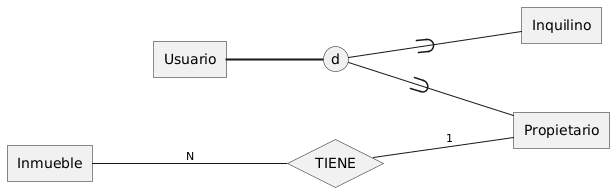
\includegraphics[width=1\linewidth]{img/db_image.png}
    \caption{Diagrama relacional de la base de datos.}
    \label{fig:placeholder}
\end{figure}